\documentclass[thesis.tex]{subfiles}

\begin{document}
\iffulldocument\else
	\chapter{KdV5}
\fi

\section{Overview}

The Kawahara equation, also known as a fifth-order KdV-type equation, is used as a model for capillary-gravity water waves, magneto-acoustic waves, plasma waves, and other dispersive phenomena. This equation takes the general form
\begin{equation}\label{kawahara}
u_t + \alpha u_{xxx} + \beta u_{xxxxx} = \frac{\partial}{\partial x} f(u, u_x, u_{xxx}),
\end{equation}
where $u(x, t)$ is a real-valued function, the parameters $\alpha$ and $\beta$ are real with $\beta \neq 0$, and $f$ is a smooth function \cite{Bridges2002,Bridges2002a}. If $f$ is a variational derivative, then \cref{kawahara} is the Hamiltonian system
\[
\partial_t u = \calJ \calE'(u),
\]
where $\calJ = \partial_x$ is skew-Hermitian, and the energy $\calE$ is given by
\begin{equation}\label{kawaharaE}
\calE(u) = -\frac{1}{2}\int_{-\infty}^\infty 
\left( \frac{1}{2}u_{xx}^2 - \frac{1}{2}\alpha u_x^2 + h(u, u_x, u_{xx})\right)dx,
\end{equation}
and $f$ in \cref{kawahara} is the variational derivative of the term involving $h$ in \cref{kawaharaE} \cite{Bridges2002}.

One specific example is the PDE
\begin{equation}\label{capgrav}
u_t + \frac{2}{15} \beta u_{xxxxx} - b u_{xxx}
+ 3 u u_x + 2 u_x u_{xx} + u u_{xxx} = 0,
\end{equation}
which is a weakly nonlinear long-wave approximation to the classical capillary-gravity water wave problem \cite{Sandstede2013,Champneys1997,Champneys1998}. Equation \cref{capgrav} is the Kawahara equation with $\alpha = -b$, $\beta = 2/15$, and $f(u, u_x, u_{xx}) = -(\frac{3}{2}u^2 + u u_{xx} + u_x^2)$.

For simplicity, we will consider the form of the Kawahara equation from \cite{Pelinovsky2007}, which we will refer to as the 5th order KdV equation (KdV5).
\begin{equation}\label{KdV5}
u_t = u_{xxxxx} - u_{xxx} - 2 u u_x .
\end{equation}
This is the Kawahara equation with $\alpha = 1$, $\beta = -1$, and $f(u, u_x, u_{xx}) = u^2$.

We are interested in traveling wave solutions, which are solutions of the the form $u(x, t) = u(x - ct)$. Writing \cref{KdV5} in a co-moving frame with speed $c$ by letting $\xi = x - ct$, equation \cref{KdV5} becomes
\begin{equation}\label{KdV5c}
u_t = \partial_x(u_{xxxx} - u_{xx} - u^2 + cu) ,
\end{equation}
where we have renamed the independent variable back to $x$. Equation \cref{KdV5c} is Hamiltonian, and can be written as $u_t = \partial_x \calE'(u)$, where $\calE(u)$ is the energy
\begin{equation}\label{KdV5energy}
\calE(u) = -\int_{-\infty}^{\infty} \left( \frac{1}{2}u_{xx}^2 + \frac{1}{2}u_x^2 + \frac{1}{2}cu^2 - \frac{1}{3}u^3 \right) dx.
\end{equation}
For any solution $u(x, t)$ to \cref{KdV5c}, the energy $\calE(u)$ is conserved in $t$. Since $\calE(u)$ only depends on the independent variable $x$ via $u(x)$, the energy is translation invariant. Finally, $\calE(u)$ is reversible, i.e. is invariant under the transformation $x \mapsto -x$.

An equilibrium solution to \cref{KdV5} satisfies the 5th order nonlinear ODE
\begin{equation}\label{KdV5eq}
u_{xxxxx} - u_{xxx} + c u_x - 2 u u_x = 0.
\end{equation}
The background state $u = 0$ is a solution to \cref{KdV5eq}. We are interested in pulse solutions, which are localized solutions which decay exponentially to the background state at $\pm \infty$. Integrating \cref{KdV5eq} once, a pulse solution must also satisfy the 4th order ODE
\begin{equation}\label{KdV5eq4}
u_{xxxx} - u_{xx} + c u - u^2 = 0,
\end{equation}
where we take the constant of integration to be 0 since pulse solutions decay to 0. Equation \cref{KdV5eq4} is Hamiltonian, with energy given by
\begin{equation}\label{KdV5ham}
H(u, u_x, u_{xx}, u_{xxx}) = u_x u_{xxx} - \frac{1}{2}u_x^2 - \frac{1}{2}u_{xx}^2 + \frac{c}{2}u^2 - \frac{1}{3}u^3 .
\end{equation}
For any solution $u(x)$ to \cref{KdV5eq4}, the Hamiltonian $H$ is conserved in $x$. We can write \cref{KdV5eq4} in standard Hamiltonian form as the first order system in $\R^4$
\begin{equation}\label{KdV5ham2}
Q' = (J \nabla \tilde{H}) Q,
\end{equation}
where 
\begin{equation}\label{KdV5Q}
Q = (q_1, q_2, p_1, p_2) = (u, u_x, -u_{xxx} + u_x, u_{xx}),
\end{equation}
\begin{equation}
\tilde{H}(q_1, q_2, p_1, p_2) = \frac{1}{3}q_1^3 - \frac{1}{2}c q_1^2 + p_1 q_2 - \frac{1}{2}q_2^2 + \frac{1}{2}p_2^2,
\end{equation}
and $J$ is the standard $4 \times 4$ symplectic matrix
\[
J = \begin{pmatrix}
0 & I_2 \\ -I_2 & 0
\end{pmatrix},
\]
where $I_2$ is the $2\times 2$ identity matrix. This form is particularly useful for numerical analysis.

Linearization of the 4th order ODE \cref{KdV5eq4} about a solution $u^*(x)$ is the self-adjoint linear operator
\begin{equation}\label{KdV5hessian}
\calE''(u^*) = \partial_x^4 - \partial_x^2 + c - 2 u^* 
\end{equation}
where $\calE''(u^*)$ is the Hessian of the energy \cref{KdV5energy}. For the rest state $u^* = 0$, the eigenvalues of $\calE''(u^*)$ are the solutions to the fourth-order polynomial equation $\nu^4 - \nu^2 + c = 0$, which are
\begin{align*}
\nu = \pm \sqrt{ \frac{1 \pm \sqrt{1 - 4c} }{2}}.
\end{align*}
For $c > 0$, two eigenvalues have positive real part and two have negative real part, thus $u = 0$ is a hyperbolic equilibrium with a two-dimensional stable manifold and a two-dimensional unstable manifold. For $0 < c < 1/4$, all four eigenvalues are real. A bifurcation takes place at $c = 1/4$, and for $c > 1/4$, the eigenvalues of $\calE''(0)$ are a quartet $\pm \alpha_0 \pm \beta_0 i$, where $\alpha_0, \beta_0 > 0$. This is shown in \cref{fig:kdv5eigbif}.

\begin{figure}[H]
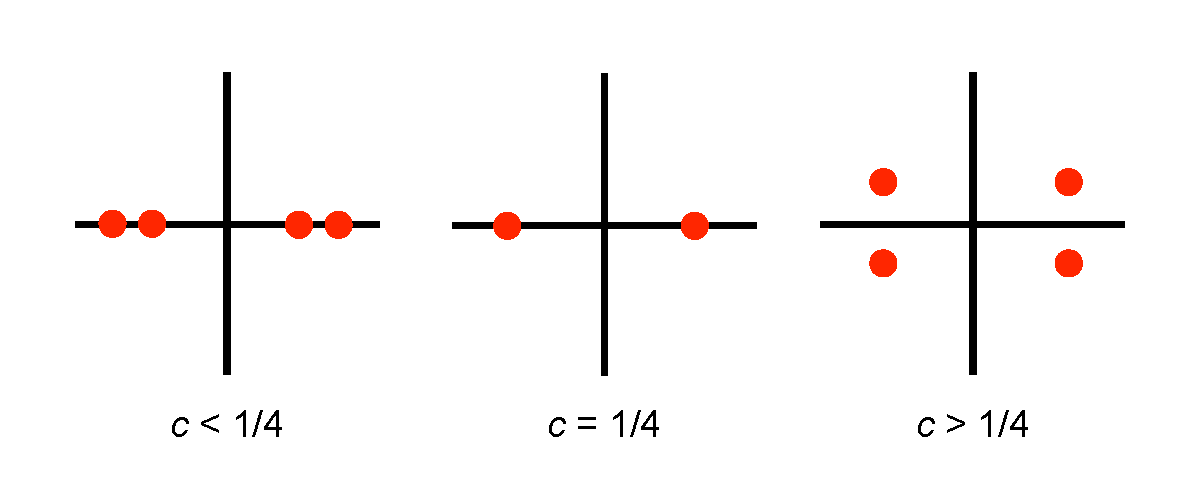
\includegraphics[width=10cm]{images/kdv5/A0eigbifurcation}
\caption[Eigenvalues of rest state for KdV5]{Eigenvalue pattern for linearization of \cref{KdV5eq4} about the rest state $u = 0$. }
\label{fig:kdv5eigbif}
\end{figure} 

As a first step to studying the stability of an equilibrium solution $u^*$, we will study the spectrum of the linearization of the PDE \eqref{KdV5c} about $u^*$. Substituting the standard linearization ansatz $u(x, t) = u^*(x) + \epsilon e^{\lambda t} v(x)$ into \eqref{KdV5c} and keeping terms up to order $\epsilon$, we obtain the PDE eigenvalue problem
\begin{equation}\label{KdV5PDEevp}
\partial_x \calE''(u^*) v = \lambda v.
\end{equation}
where $\calE''(u^*): H^4(\R) \subset L^2(\R) \rightarrow L^2(\R)$ is given in \cref{KdV5hessian}.

\section{Primary pulse solution}

For $c > 0$, a symmetric one-pulse solution exists to \cref{KdV5eq4}. We will refer to this as the primary pulse solution. This result is stated in the following theorem, which is adapted from \cite[Theorem 2.1]{Pelinovsky2007}. The proof uses a mountain-pass argument.

\begin{theorem}[Existence of Primary Pulse]\label{KdV1pulse}
For $c > 0$, there exists a one-pulse solution $q(x)$ to \cref{KdV5eq4} which is an even function and decays exponentially to 0 at $\pm \infty$. For the linear operators $\calE''(q)$ and $\partial_x \calE''(q)$, we have the following:
\begin{enumerate}[(i)]
\item The linear operator $\calE''(q)$ has exactly one negative eigenvalue with an even eigenfunction and a simple eigenvalue at 0 with eigenfunction $q_x$.
\item Assume that the map $c \mapsto q(x; c)$ is $C^1$ for $c > 0$. Then the linear operator $\partial_x \calE''(q)$ has an eigenvalue at 0 with algebraic multiplicity 2 and geometric multiplicity 1; the eigenfunction is $\partial_x q(x)$ and the generalized eigenfunction is $\partial_c q(x)$. 
\item Assume that 
\[
\frac{\partial}{\partial c} \left( \frac{1}{2} \int_{-\infty}^\infty q(x)^2 dx \right) > 0
\]
Then $q(x)$ is orbitally stable. This implies that $\partial_x \calE''(q)$ has no eigenvalues with positive real part.
\end{enumerate}
\end{theorem}

\section{Multi-pulse solutions}

For $c > 1/4$, multi-pulse solutions exist to \cref{KdV5eq4}. These resemble multiple, well-separated copies of the primary pulse $q(x)$. For each $n \geq 2$, Buffoni, Champneys, and Toland \cite{Buffoni1996} show that a countable family of multi-pulse solutions exists; their proof uses the Smale horseshoe set. The result for 2-pulse solutions is also given in \cite[Theorem 2.2]{Pelinovsky2007}, which is based on the variational method used in \cite{Buffoni1996}. 

The method we will use is due to Sandstede \cite{Sandstede1993,SandstedeStrut} using spatial dynamics and Lin's method. The distances between consecutive pulses are constrained to be (approximately) an integer multiple of a phase parameter which depends on $\beta_0$. Geometrically, these integers represent the number of half-twists made by the multi-pulse between consecutive peaks. As discussed briefly in \cref{chapter:intro}, a specific alignment of stable and unstable manifolds necessary for multi-pulses to exist. We will state the existence result using this method in \cref{chapter:kdv5multi}, which is a straightforward adaptation of \cite[Theorem 3.6]{SandstedeStrut}. 

\section{Spectrum of multi-pulses}

We now look at the spectral stability of multi-pulses. Let $q_n$ be an $n-$pulse equilibrium solution to \cref{KdV5c}. We are interested in the spectrum of the linear operator $\partial_x \calE''(q_n): H^5(\R) \subset L^2(\R) \rightarrow L^2(\R)$, which is the set of $\lambda \in \C$ for which the operator $\partial_x \calE''(q_n) - \lambda \calI$ does not have bounded inverse. The spectrum can be divided into two parts. The essential spectrum consists of the set of all $\lambda \in \C$ for which the operator $\partial_x \calE''(q_n) - \lambda \calI$ either is not Fredholm or is Fredholm with nonzero inedx. The point spectrum is the set of all $\lambda$ for which $\partial_x \calE''(q_n) - \lambda \calI$ is Fredholm with index 0 but is not invertible. An eigenvalue is an element of the point spectrum. For KdV5, it follow from \cite[Theorem 3.1.11]{Kapitula2013} that $\partial_x \calE''(q_n) - \lambda \calI$ cannot be Fredholm with nonzero index. Thus the essential spectrum consists of all $\lambda \in \C$ for which the operator $\partial_x \calE''(q_n) - \lambda \calI$ is not Fredholm and the point spectrum consists of all $\lambda \in \C$ for which $\dim \ker(\partial_x \calE''(q_n) - \lambda \calI) > 0$.

It it straightforward to show that 
\begin{align*}
\partial_x \calE''(q_n) (\partial_x q_n) &= 0 \\
\partial_x \calE''(q_n) (-\partial_c q_n) &= \partial_x q_n
\end{align*}
Thus there is an eigenvalue at 0 with at least algebraic multiplicity 2 and geometric multiplicity 1. The kernel eigenvalue $\partial_x q_n$ is a consequence of translation invariance. For the essential spectrum, since $\partial_x \calE''(q_n)$ is exponentially asymptotic to the operator 
\[
\partial_x \calE''(0) = 
\partial_x(\partial_x^4 - \partial_x^2 + c - 2 u^*),
\]
by the Weyl essential spectrum theorem \cite[Theorem 2.2.6]{Kapitula2013} and \cite[Theorem 3.1.11]{Kapitula2013}, $\partial_x \calE''(q_n)$ and $\partial_x \calE''(0)$ have the same essential spectrum. By a straightforward calculation, the essential spectrum of $\partial_x \calE''(q_n)$ is the entire imaginary axis.

All that remains is to locate the rest of the point spectrum. We expect that, as in \cite{Sandstede1998}, the $n-$pulse $q_n$ will have $n-1$ additional sets of eigenvalues near 0. We will call these interaction eigenvalues since they result from interactions between neighboring pulses. Since \cref{KdV5c} is Hamiltonian, these interaction eigenvalues must come in quartets $\{ \pm \lambda, \pm \overline{\lambda}\}$ \cite[Proposition 5.1.2]{Kapitula2013}. Thus each set of eigenvalues must come in one of the three patterns in \cref{fig:kdv5inteigpattern}.

\begin{figure}[H]
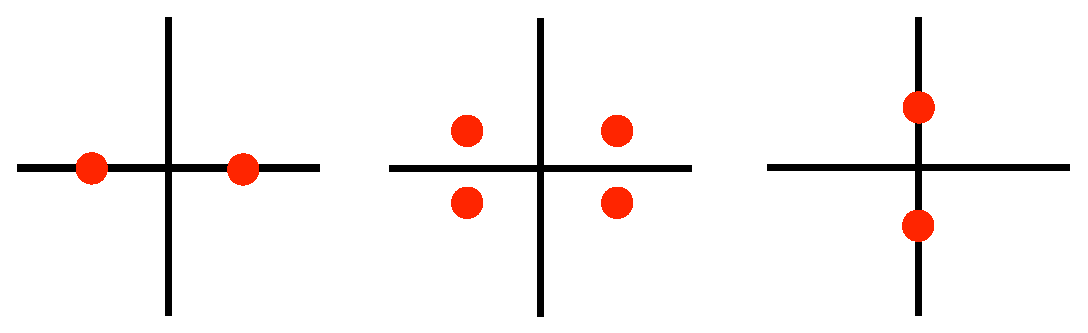
\includegraphics[width=10cm]{images/kdv5/eigdouble2}
\caption[Possible interaction eigenvalue patterns for KdV5]{Possible interaction eigenvalue patterns for multi-pulses for KdV5. The first two patterns are unstable. The third pattern is neutrally stable.}
\label{fig:kdv5inteigpattern}
\end{figure}

\noi By Hamiltonian symmetry, the presence of an eigenvalue with nonzero real part implies that there is an unstable eigenvalue with positive real part. Thus the best we can hope for is neutral stability. For double pulses, Chugunova and Pelinovsky prove that there is a pair of interaction eigenvalues with is either real or purely imaginary (to leading order) with negative Krein signature \cite[Theorem 2.3]{Pelinovsky2007}. 

The presence of the essential spectrum along the entire imaginary axis makes any purely imaginary interaction eigenvalues difficult to locate. In \cref{chapter:kdv5multi}, we will use an exponentially weighted space to move the essential spectrum into the left half plane. This will allow us to obtain a result for the spectrum of multi-pulses. However, as in \cite{Pelinovsky2007}, we will only be able to prove that eigenvalues close to the imaginary axis are purely imaginary to leading order. Thus while we can obtain an instability result, we cannot obtain a stability result. Another way to simplify the problem is to look at periodic solutions. On a periodic domain, the essential spectrum becomes a discrete set of eigenvalues, which in principle makes the analysis more straightforward. We look at the existence of multi-pulses on a perioidic domain in \cref{chapter:kdv5multi}, but their spectral stability remains unknown.

\iffulldocument\else
	\bibliographystyle{amsalpha}
	\bibliography{thesis.bib}
\fi

\end{document}